\documentclass[12pt,titlepage]{article}
\usepackage[margin=1.25in]{geometry}
\usepackage{graphicx,amsmath,blindtext}

%% Variables definition
\newcommand{\vSubject}{Basic Programming}
\newcommand{\vSubtitle}{Looping Exercise}
\newcommand{\vName}{Dicha Zelianivan Arkana}
\newcommand{\vNIM}{2241720002}
\newcommand{\vClass}{1i}
\newcommand{\vDepartment}{Information Technology}
\newcommand{\vStudyProgram}{D4 Informatics Engineering}

%% [START] Tikz related stuff
\usepackage{tikz}
\usetikzlibrary{svg.path,calc,shapes.geometric,shapes.misc}
\tikzstyle{terminator} = [rectangle, draw, text centered, rounded corners = 1em, minimum height=2em]
\tikzstyle{preparation} = [chamfered rectangle, chamfered rectangle sep=0.75em, draw, text centered, minimum height = 2em]
\tikzstyle{process} = [rectangle, draw, text centered, minimum height=2em]
\tikzstyle{decision} = [diamond, aspect=2, draw, text centered, minimum height=2em]
\tikzstyle{data}=[trapezium, draw, text centered, trapezium left angle=60, trapezium right angle=120, minimum height=2em]
\tikzstyle{connector} = [line width=0.25mm,->]
%% [END] Tikz related stuff

%% [START] Fancy header related stuff
\usepackage{fancyhdr}
\pagestyle{fancy}
\setlength{\headheight}{15pt} % compensate fancyhdr style
\fancyhead{}
\fancyfoot{}
\fancyfoot[L]{\thepage}
\fancyfoot[R]{\textit{\vSubject - \vSubtitle}}
\renewcommand{\footrulewidth}{0.4pt}% default is 0pt, overline for footer
%% [END] Fancy header related stuff

%% [START] Custom tabular command related stuff
\usepackage{tabularx}
\newcommand{\details}[2]{
    #1 & #2  \\
}
%% [END] Custom tabular command related stuff

%% [START] Figure related stuff
\newcommand{\image}[3][1]{
    \begin{figure}[h]
        \centering
        \includegraphics[#1]{#2}
        \caption{#3}
        \label{#3}
    \end{figure}
}
%% [END] Figure related stuff

\begin{document}
\begin{titlepage}
    \centering
    \vfill
    {\bfseries\LARGE
        \vSubject\\
        \vskip0.25cm
        \vSubtitle
    }
    \vfill
    
\includegraphics[width=6cm]{images/polinema-logo.png}
    \vfill
    {
        \textbf{Name}\\
        \vName\\
        \vskip0.5cm
        \textbf{NIM}\\
        \vNIM\\
        \vskip0.5cm
        \textbf{Class}\\
        \vClass\\
        \vskip0.5cm
        \textbf{Department}\\
        \vDepartment\\
        \vskip0.5cm
        \textbf{Study Program}\\
        \vStudyProgram
    }
\end{titlepage}

\section*{Exercise}
Create a flowchart from the following problems using for, while, and do-while!
\begin{enumerate}
    \item {
        Displays the odd number from 11 to 188

        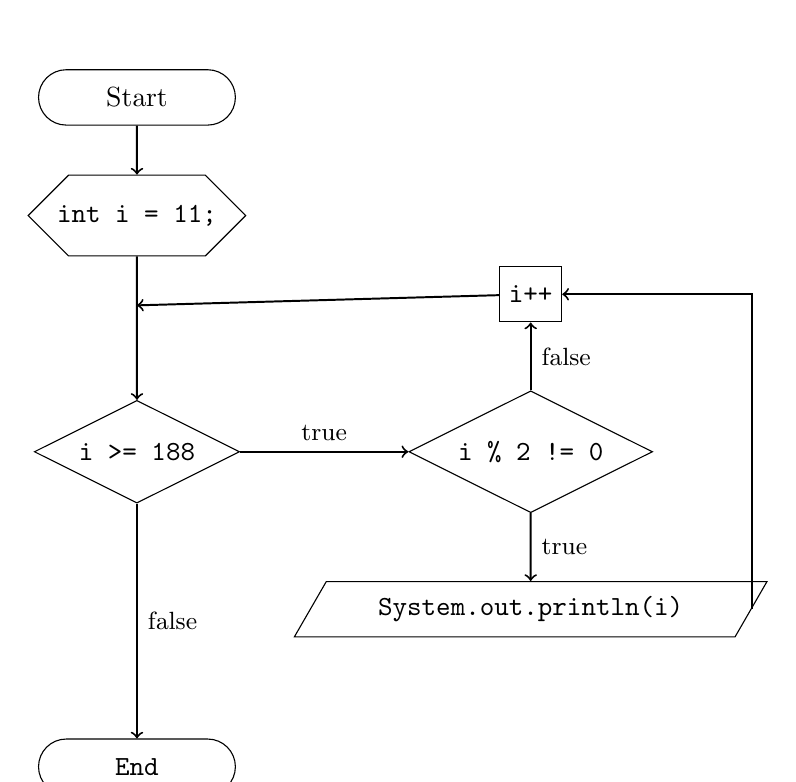
\begin{tikzpicture}
            \centering
            \node (start) [terminator, align=center, minimum width=2.5cm] {Start};
            \node (prep) [preparation, below of = start, yshift = -5mm] {\texttt{int i = 11;}};
            \node (cond) [decision, below of = prep, yshift = -2cm] {\texttt{i >= 188}};
            \node (cond2) [decision, right of = cond, xshift = 4cm] {\texttt{i \% 2 != 0}};
            \node (print) [data, below of = cond2, yshift = -1cm] {\texttt{System.out.println(i)}};
            \node (increment) [process, above of = cond2, yshift=1cm] {\texttt{i++}};
            \node (end) [terminator, align=center, minimum width=2.5cm, below of = cond, yshift = -3cm] {\texttt{End}};
            \draw [connector] (start) -- (prep);
            \draw [connector] (prep) -- (cond);
            \draw [connector] (cond) -- node[right=0.1mm] {\small{false}} (end);
            \draw [connector] (cond) -- node[above=0.1mm] {\small{true}} (cond2);
            \draw [connector] (cond2) -- node[right=0.1mm] {\small{true}} (print);
            \draw [connector] (cond2) -- node[right=0.1mm] {\small{false}} (increment);
            \draw [connector] (print.east) |- (increment.east);
            \draw [connector] (increment) -- ($(cond.north)-(0,-12mm)$);
        \end{tikzpicture}
    }
    \pagebreak
    \item {
        Displays the sum of the series of numbers 1 to 30

        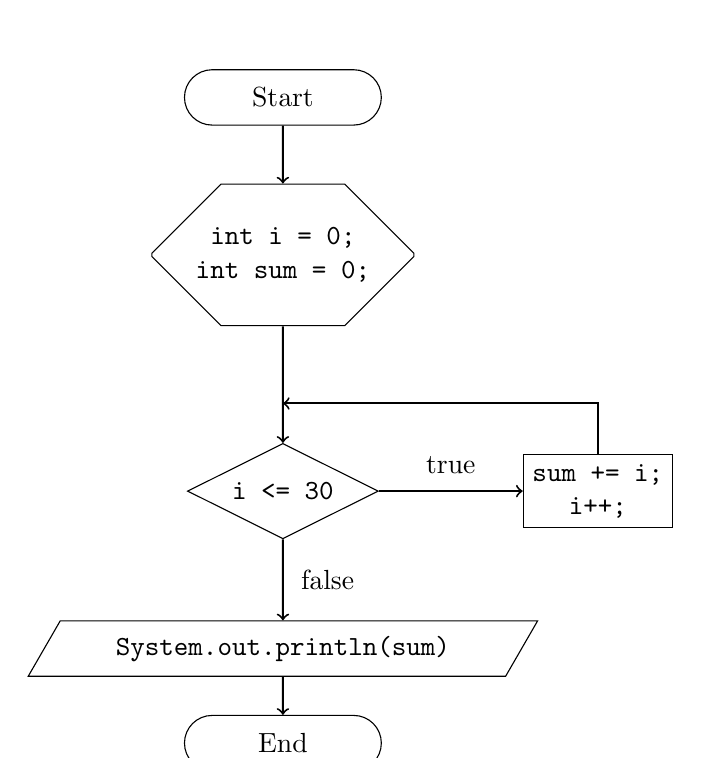
\begin{tikzpicture}
            \centering
            \node (start) [terminator, align=center, minimum width=2.5cm] {Start};
            \node (prep) [preparation, below of = start, yshift = -1cm, align=center, chamfered rectangle sep=1.25em] {
                \texttt{int i = 0;}\\
                \texttt{int sum = 0;}
            };
            \node (cond) [decision, below of = prep, yshift = -2cm] {\texttt{i <= 30}};
            \node (add) [process, right of = cond, xshift = 3cm, align=center] {
                \texttt{sum += i;}\\
                \texttt{i++;}
            };
            \node (print) [data, below of = cond, yshift = -1cm] {\texttt{System.out.println(sum)}};
            \node (end) [terminator, align=center, minimum width=2.5cm, below of = print, yshift = -2mm] {End};
            \draw [connector] (start) -- (prep);
            \draw [connector] (prep) -- (cond);
            \draw [connector] (cond) -- node[above=1mm] {true} (add);
            \draw [connector] (cond) -- node[right=1mm] {false} (print);
            \draw [connector] (add.north) |- ($(cond.north)-(0,-5mm)$);
            \draw [connector] (print) -- (end);
        \end{tikzpicture}
    }
    \pagebreak
    \item {
        Calculates the power of $X^Y$ with X and Y from the user input

        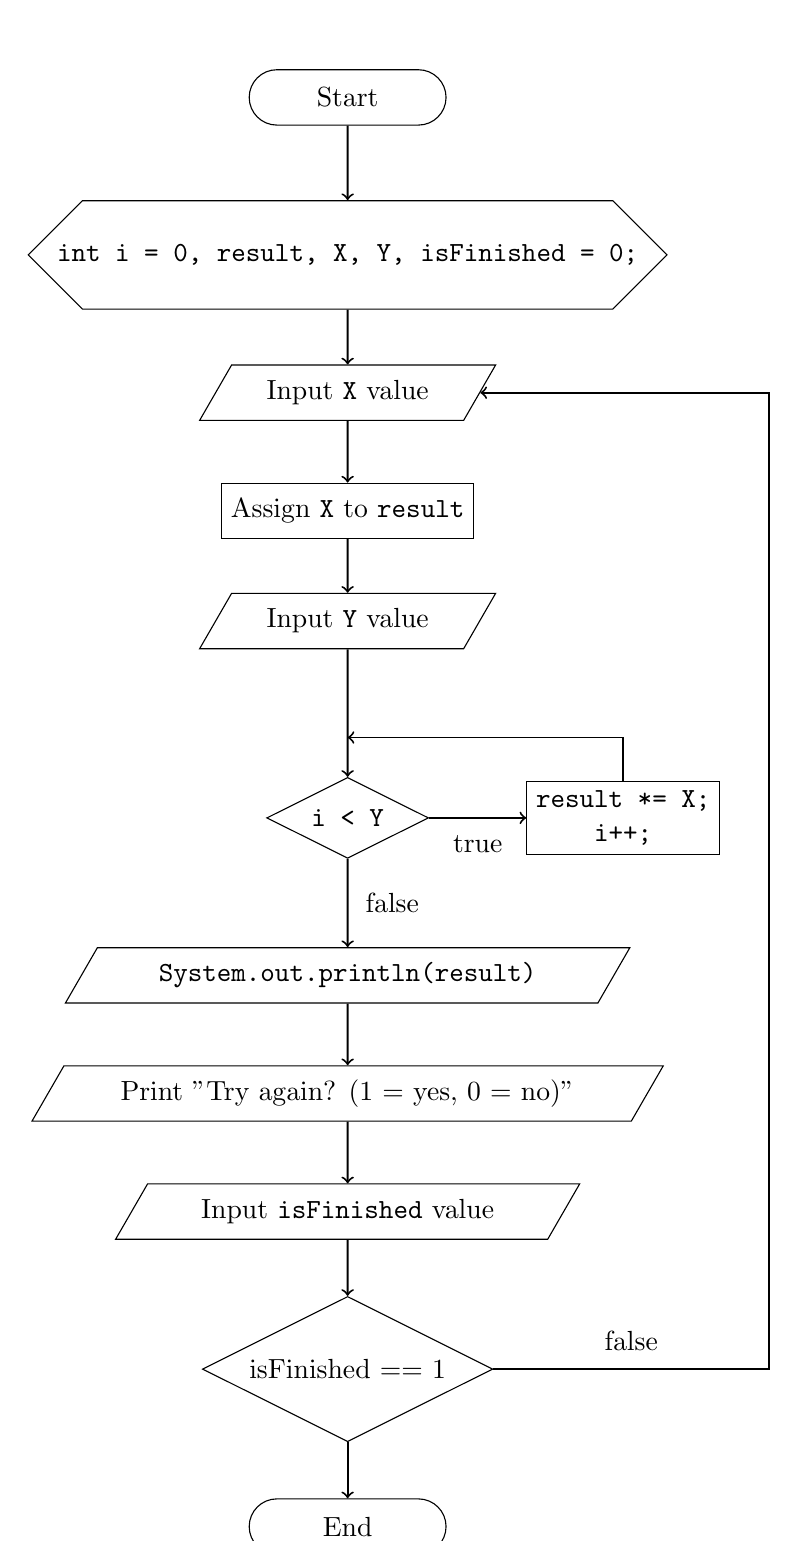
\begin{tikzpicture}
            \centering
            \node (start) [terminator, align=center, minimum width=2.5cm] {Start};
            \node (prep) [preparation, below of = start, yshift = -1cm, align=center, chamfered rectangle sep=1.25em] {\texttt{int i = 0, result, X, Y, isFinished = 0;}};
            \node (inputX) [data, below of = prep, yshift = -7.5mm] {Input \texttt{X} value};
            \node (assign) [process, below of = inputX, yshift = -5mm] {Assign \texttt{X} to \texttt{result}};
            \node (inputY) [data, below of = assign, yshift = -4mm] {Input \texttt{Y} value};
            \node (cond-pow) [decision, below of = inputY, yshift = -1.5cm] {\texttt{i < Y}};
            \node (pow) [process, right of = cond-pow, xshift = 2.5cm, align=center] {
                \texttt{result *= X;}\\
                \texttt{i++;}
            };
            \node (print) [data, below of = cond-pow, yshift = -1cm] {\texttt{System.out.println(result)}};
            \node (printQuestion) [data, below of = print, yshift = -5mm] {Print "Try again? (1 = yes, 0 = no)"};
            \node (inputAnswer) [data, below of = printQuestion, yshift = -5mm] {Input \texttt{isFinished} value};
            \node (cond) [decision, below of = inputAnswer, yshift = -1cm] {isFinished == 1};
            \node (end) [terminator, align=center, minimum width=2.5cm, below of = cond, yshift = -1cm] {End};
            \draw [connector] (start) -- (prep);
            \draw [connector] (prep) -- (inputX);
            \draw [connector] (inputX) -- (assign);
            \draw [connector] (assign) -- (inputY);
            \draw [connector] (inputY) -- (cond-pow);
            \draw [connector] (cond-pow) -- node[right=1mm] {false} (print);
            \draw [connector] (cond-pow) -- node[below=1mm] {true} (pow);
            \draw [connector] (pow.north) |- ($(cond-pow.north)+(0,5mm)$);
            \draw [connector] (print) -- (printQuestion);
            \draw [connector] (printQuestion) -- (inputAnswer);
            \draw [connector] (inputAnswer) -- (cond);
            \draw [connector] (cond.east) -- node[above=1mm] {false} ($(cond.east)+(3.5cm,0)$) |- (inputX.east);
            \draw [connector] (cond) -- (end);
        \end{tikzpicture}
    }
    \pagebreak
    \item {
        Displays a series of numbers 2 4 8 16 32… 256

        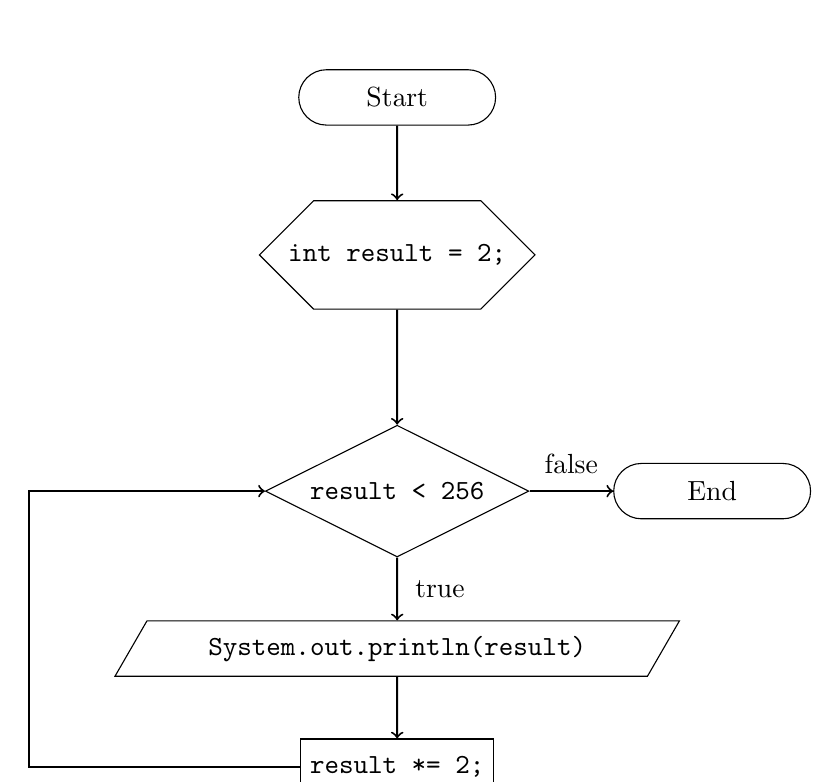
\begin{tikzpicture}
            \centering
            \node (start) [terminator, align=center, minimum width=2.5cm] {Start};
            \node (prep) [preparation, below of = start, yshift = -1cm, align=center, chamfered rectangle sep=1.25em] {\texttt{int result = 2;}};
            \node (cond) [decision, below of = prep, yshift = -2cm] {\texttt{result < 256}};
            \node (print) [data, below of = cond, yshift = -1cm] {\texttt{System.out.println(result)}};
            \node (add) [process, below of = print, yshift = -5mm, align=center] {\texttt{result *= 2;}};
            \node (end) [terminator, align=center, minimum width=2.5cm, right of = cond, xshift = 3cm] {End};
            \draw [connector] (start) -- (prep);
            \draw [connector] (prep) -- (cond);
            \draw [connector] (cond) -- node[right=1mm] {true} (print);
            \draw [connector] (add.west) -| ($(cond.west)-(3cm,0)$) -- (cond.west);
            \draw [connector] (print) -- (add);
            \draw [connector] (cond) -- node[above=1mm] {false} (end);
        \end{tikzpicture}
    }
\end{enumerate}

\end{document}

